\chapter{Renderering}

在渲染方面上的研究与优化已经发展成熟,已成为一个非常复杂的系统了,本文的目标是从理解渲染的技术原理,从软渲染,到CPU,再到GPU。
为简化,我们以图元三角形为例,主要有两个阶段:
\begin{itemize}
    \item {决定那些像素坐标构成这个三角形}
    \item {决定这些像素的颜色值是多少,这个过程就是着色shading}
\end{itemize}
它们分别对应着图形学中另外两个概念,光栅化和光照模型。

\section{Rasterize}
光栅化
图形学中,是物理的三维世界,如何把三维物体在二维屏幕上显示,需要把它的三维属性都降为二维的结果,大致存在以下几个步骤:

\begin{itemize}
    \item {坐标变换}
    \item {属性计算,如颜色,纹理,alpha等}
    \item {光栅化}
\end{itemize}

\textsf{目前大众屏幕分辨率为1920x1080,在二维屏幕渲染时,内存中的FrameBuffer只保存着1920x1080个屏幕点的颜色,然后再映射到屏幕上面。
光栅化的,就是计算出1920x1080个点的颜色值的过程。把物体的数学描述转换为屏幕的像素值,是从连续到离散,即物理的坐标是浮点数,而屏幕坐标是整数,光栅化的过程是一个近似的过程。
在一些图形处理软件中就是把矢量图形转化成像素点的过程。}

\begin{description}
    \item [主动:] \textsf{定时渲染,与时间关系比较严格的}
    \item [被动:] \textsf{请求渲染,与动画相关的,以流畅为结果}
\end{description}

\text{目前处理光照生成图像的过程中,计算的级别有:}

\begin{itemize}
    \item {逐顶点光照,在每个顶点计算光照,在渲染图元内部进行插值,光照模型中的非线性关系会产生问题}
    \item {逐像素光照,Phong着色,在fragment对顶点法线进行插值}
\end{itemize}


\section{Photorealistic Rendering}

真实感图形技术包括消隐技术,光照模型,明暗处理和纹理,阴影生成等

\begin{itemize}
    \item {局部光照,仅处理光源直接照射物体表面的光照模型,与光栅化渲染算法相适应的,一次只考虑
    一个像素的光照强度,逐像素的光照计算,不能得到其他像素的光照影响值}
    \begin{itemize}
        \item {Lambert漫反射模型,不能很好处理镜面与高光}
        \item {Gourand}
        \item {Phong,支持高光与镜面}
        \item {Blinn-Phong,速度快,目前商业普遍使用}
        \item {Cook-Torrance,以双向反射的基础上}
    \end{itemize}
    \item {全局光照,基于光学物理原理,光照强度的计算依赖于光能在现实世界中的传播,考虑光线与整个场景中
    各物体表面以及物体表面之间的相互影响,包括多次反射、透射、散射等,成熟应用在离线渲染中}
    \begin{itemize}
        \item {光线跟踪,模拟光从光源出发经过若干次反射、折射达到摄像机的过程,由于只有最终到达摄像机的光线
        才对生成图像有贡献,实现中是以摄像机逆向发出光线,以寻求达到光源的路径。}
        \begin{itemize}
            \item {路径跟踪Path Tracing}
            \item {递归光线追踪Whitte-type}
            \item {分布式光线追踪Distrubution}
            \item {双向路径追踪Bidirectional Path}
            \item {Metropolis}
        \end{itemize}
        \item {辐射度算法,是一种物体空间的算法,用于解离散点或环境中表面曲面面片的光强度问题,而不是解图像平面
        投影的像素问题}
        \item {光子映射,改善漫反射辉映,焦散等全局光照效果,还无法应用在实时渲染中}
    \end{itemize}
\end{itemize}

\section{Non-Photorealistic Rendering}
对于某些场景,不需要真实感,需要一些艺术化的表现
钢笔素描的生成,
中国国画与书法的生成。
\newline
\textbf{Artistic Shading},艺术渲染,模拟人简画的素描之类的,是一种根据轮廓来来抽象效果。

\section{Image-Based Rendering}

IBR,基于图像的渲染,完全摒弃传统的先建模,然后确定光源的渲染方法,
它直接从一系列已知的图像中生成新颖的视口图像,适用于野外极其复杂场景的生成和漫游。

\section{Stereo Rendering}
立体渲染,是一种让人眼能够感受到立体效果的渲染方式,需要两个camera对同一个场景进行渲染,两个view得到
的图像略有差异(两个camera的投影矩阵的差异),让人产生深度的视觉效果。一般分左右两个camera。

通常渲染完成后,整张图像还需要一次后处理Barrel distortion桶形失真,以抵消VR设备固有的pincushion distortion枕形失真。
\begin{figure}[h]
    \centering
    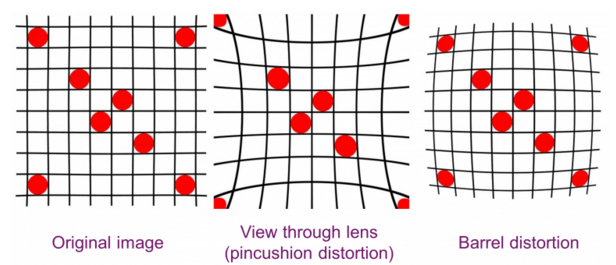
\includegraphics[width=\textwidth]{images/Optimising-OpenGL-ES-for-mobile-VR-lens-distortion.png}
    \caption{Phong Shading Model}
\end{figure}


\section{Deferred Shading}

\begin{itemize}    
    \item {不能使用混合技术}
    \item {占用较高的显存}
    \item {光照的开销与场景复杂度无关}
    \item {Shader可以访问深度和其他像素信息}
    \item {每个像素对每个光源仅运行一次,被遮挡的像素是不会参与计算}
    \item {材质与光照的Shader是分开的}
\end{itemize}

\section{Anti-Aliasing}

渲染中,最终结果是一张图像,其最小单位就是像素。像素是很小的一个色块,当图像分辨率足够高时,色块足够小,
相邻色块之间的颜色差异人眼是很难辨别的,看到的就是一副细腻顺滑的图像,当分辨率较低时,为了填充同样大小的
屏幕,色块的尺寸就相应变大了,色块之间的差异就很难被忽视了。因为屏幕是点阵显示,就造成物理上无法避免的问题。

\subsection{Samping}

锯齿产生的主要情况有:
\begin{itemize}
    \item {几何走样,几何物体的边缘有锯齿,对几何边缘采样不足导致的}
    \item {着色走样,渲染方程中的着色公式采样不足导致的,就是高光闪烁就是一种情况}
    \item {时间走样,对高速物体的采样不足,比如播放的动画发生跳变}
\end{itemize}

按照香农采样定律的理论,要想通过对采样后的信号进行重建Reconstruct来获得原始信号,就必须保证采样频率不低于
原始信号最高频率的两倍。

\begin{figure}[h]
    \centering
    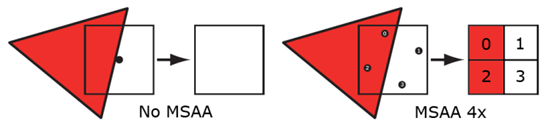
\includegraphics[width=\textwidth]{images/ssaa.png}
    \caption{SuperSampling AA}
\end{figure}

图元覆盖在色块上,简单的判断就是是否中心点被覆盖否,但是这样判断会引入图元的位置差异结果,将色块进一步细分成不同的
小块,对每个小块进行判断,再由这些小块的颜色加权计算出来,这就是通过采样来得到更好的颜色值。

带来的问题就是一次pass对Pixel/Fragment shader需要4倍的像素处理,另一种思路就是多次pass的Accumulation Buffer方法,
每次pass时都进行一定程度的偏移(通常0.5个像素),最后进行累积后再平均,但是多次绘制需要进行Buffer之间的
数据拷贝,消耗也是非常大的。


\subsection{Sampling Pattern}

先说说采样点纹,即才采样点在像素色块中的分布方式。研究表明人眼感官影响最严重的锯齿现象是由水平或垂直边缘导致的,其次是45度夹角的边缘。
Rotated Grid SuperSampling就是把采样点旋转45度的来提升AA的质量。

\subsection{MSAA}

Multisampling Antialiasing是改进版,SSAA对每次FS需要四次sample计算,假设色块任意点颜色值近似相同,把sample后的值存入
对应的buffer中,利用这些覆盖点的sample点进行插值,就是Centroid Sampling(Interplotation),这个动作通常由硬件自动完成。

MSAA渲染完成后,需要将subsample的数据转换为pixel color,这个过程称为MSAA 解析Resolve。现代GPU的FS或Compute Shader都可以直接
操作MSAA的处理过程,可以使用不同的filter来实现图像的AA重建,可以参考\cite{OpenGLMultiSampling}

下图来自Direct3D11的Graphics Pipeline\cite{RasterizationRules} 

\begin{figure}[h]
    \centering
    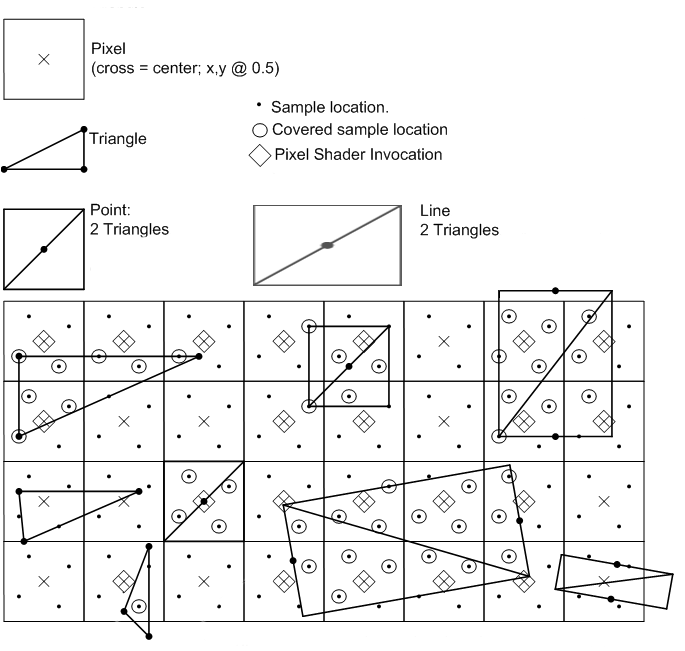
\includegraphics[width=\textwidth]{images/d3d10-rasterrulesmsaa.png}
    \caption{MSAA sample 4 for d3d10}
\end{figure}

\subsection{TAA}

上面讨论的都是在同一帧中,像素在不同位置上的采样处理,可认为是空间上的方法。现在从时间角度上来分析,实时渲染在一秒内会进行
多帧的连续渲染,前后两帧的重复度极高,利用之前多帧的渲染结果提取信息来优化渲染结果是否可行呢?这就是Temporal AA。 

使用TAA好处是同一帧没有额外的采样消耗,只需要对多帧结果进行一个融合即可,但多帧的重叠度与加权值的处理不够好时,会出现抖动闪烁
的瑕疵。解决方法有两种,一是只对低速物体使用TAA,一是对当前帧与之前帧的画面进行映射与投影校正reprojection,常见的使用速度
贴图velocity buffer。TAA+Velocity Buffer与Deferred Rendering是不兼容的。

\subsection{MLAA}

锯齿产生在于几何形状与颜色交界处,如果能事先得到这些信息,就可以针对性的进行抗锯齿处理,2019年Reshetov提出一种沿着边界线
edge进行的AA方法,称为Morphological Antialiasing, 此方法侧重于边界线的定位与重构。

